% file: sections/bicomp-dfs-tree.tex

\documentclass[tikz]{standalone}
\usepackage{tikz-qtree}

\begin{document}
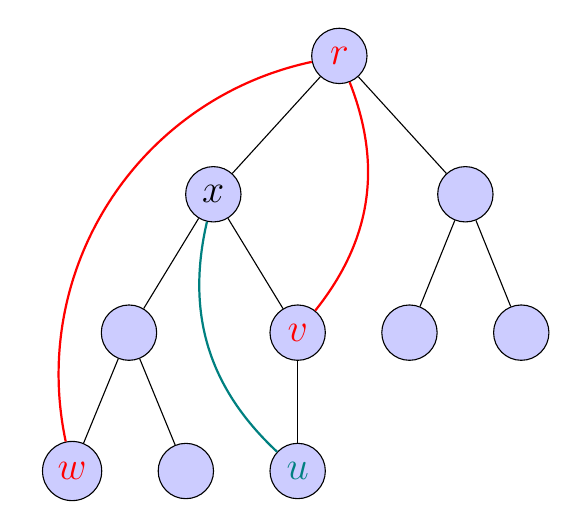
\begin{tikzpicture} [level distance = 50pt, sibling distance = 20pt,
  edge from parent/.style= { % added code
      draw, edge from parent path = {(\tikzparentnode) -- (\tikzchildnode)}}]
  \tikzset{every tree node/.style = 
    {align = center, circle, draw, fill = blue!20, font = \Large, minimum size = 20pt}}
    \Tree [.\textcolor{red}{$r$}
	    [.\node (l) {$x$};
	       [.\node (ll) {};
	        \node (w) {\textcolor{red}{$w$}};
		$$
	       ]
	       [.\node (v) {\textcolor{red}{$v$}};
		 \node (u) {\textcolor{teal}{$u$}};
	       ]
            ]
	    [.$$ 
	      $$
	      $$
	    ] 
        ]

    \path (u) edge[thick, teal, bend left] (l)
	(w) edge[thick, red, bend left = 45] (r)
	(v) edge[thick, red, bend right] (r);
\end{tikzpicture}
\end{document}
